\documentclass[14pt]{article}
\usepackage{pdfpages}
\usepackage[a4paper,pdftex]{geometry}	
\usepackage{xcolor}
\usepackage{fix-cm}
\usepackage[russian]{babel}
\usepackage[utf8]{inputenc}
\usepackage{listings}

\usepackage{graphicx}
\DeclareGraphicsExtensions{.pdf,.png,.jpg}
\usepackage{wrapfig}
\renewcommand{\thefigure}{\arabic{figure}}
\renewcommand{\thetable}{\thesection.\arabic{figure}}

\definecolor{royalBlue}{rgb}{0,35,102}
  
 \lstset{ 
  basicstyle=\big
  language=R,                     % the language of the code
  basicstyle=\tiny\ttfamily, % the size of the fonts that are used for the code
  numbers=left,                   % where to put the line-numbers
  numberstyle=\tiny\color{blue},  % the style that is used for the line-numbers
  stepnumber=1,                   % the step between two line-numbers. If it is 1, each line
                                  % will be numbered
  numbersep=5pt,                  % how far the line-numbers are from the code
  backgroundcolor=\color{white},  % choose the background color. You must add \usepackage{color}
  showspaces=false,               % show spaces adding particular underscores
  showstringspaces=false,         % underline spaces within strings
  showtabs=false,                 % show tabs within strings adding particular underscores
  frame=single,                   % adds a frame around the code
  rulecolor=\color{black},        % if not set, the frame-color may be changed on line-breaks within not-black text (e.g. commens (green here))
  tabsize=2,                      % sets default tabsize to 2 spaces
  captionpos=b,                   % sets the caption-position to bottom
  breaklines=true,                % sets automatic line breaking
  breakatwhitespace=false,        % sets if automatic breaks should only happen at whitespace
  keywordstyle=\color{royalBlue},      % keyword style
  commentstyle=\color{YellowGreen},   % comment style
  stringstyle=\color{green}      % string literal style
} 



%\usepackage[T1]{fontenc}
%\usepackage{mathptmx}

\geometry{top=2cm} % отступ сверху
\geometry{bottom=2.5cm} % отступ снизу
\geometry{left=2cm} % отступ справа
\geometry{right=2cm}


\author{
Пахтусов Н. Г., ПРО-306,\\
Чекушин Г. Я., ПРО-306,\\
Видинеев В. О., ПРО-306.
}
\makeatletter
\begin{document}

\begin{center}
\thispagestyle{empty} 

Федеральное государственное бюджетное образовательное учереждение высшего \\
профессионального образования\\
<<Уфимский государственный авиационный технический университет>>
\vspace*{\fill}
\begingroup
\centering

Отчёт по лабораторной работе\\
по дисциплине: <<Статистическое моделирование>> \\
на тему: <<Оценки>>.

\endgroup
\vspace*{\fill}

\end{center}

\begin{flushright}

Выполнили:\\
\@author \\
Проверила: \\
Рассадникова Е. Ю.

\end{flushright}

\begin{center}
Уфа, 2015
\end{center}

\clearpage

\tableofcontents

\clearpage

\section{Сравнение трех способов оценивания}
\subsection{Задание}
Сравнить три способа оценивания на выборках объема n = 10, n = 40 и n = 160 для величин, распределенных по нормальному и экспоненциальному законам распределения. 
\subsection{Теория}

Будем сравнивать три способа оценки:
\begin{enumerate}
	\item Оценка, полученная методом моментов:\\
	\^a$_1$ = $\frac{2}{n} * \sum\limits_{i=1}^n x_i$,\\ где n -- количество независимых испытаний случайной величины X, x$_i$ -- значение случайной величины в i-ом испытании.
	\item Оценка, полученная методом максимального правдоподобия:
\\
	\^a$_2$ = $\frac{n + 1}{n} * MAX(x_i)$,\\ где n -- количество независимых испытаний случайной величины X, MAX(x$_i$) -- максимальное значение случайной величины.
	\item Оценка, полученная методом порядковых статистик:
	\\
	\^a$_3 = 2 * x_{0,5}$,\\ где x$_{0,5}$ -- выборочная квантиль порядка 0,5, то есть выборочная медианна. 
\end{enumerate}

\subsection{Решение}

Для нахождения оценок и их сравнения будем использовать язык <<R>>.

Создадим необходимые выборки:
\begin{itemize} 
\item для нормального распределения:
\lstset {language=R}
\begin{lstlisting}
n <- 10
varCount <- 20
foo = rnorm

xs <- foo(n*varCount)
M <- matrix(xs, varCount, n)
\end{lstlisting}

Изменяя значение n на необходимое, получим также выборки и для n = 20, и для n = 160.

вычислим значения оценок: 
\lstset {language=R}
\begin{lstlisting}
rez1 <- apply(M, 1, function(x) (2/n)*sum(x))
rez2 <- apply(M, 1, function(x) ((n+1)/n) * max(x))
rez3 <- apply(M, 1, function(x) (2*quantile(x, c(0.5))))
\end{lstlisting}

\item Для экспоненциального распределения:
\lstset {language=R}
\begin{lstlisting}
n <- 10
varCount <- 20
foo = rexp

xs <- foo(n*varCount)
M <- matrix(xs, varCount, n)
\end{lstlisting}

Изменяя значение n на необходимое, получим также выборки и для n = 20, и для n = 160.

вычислим значения оценок: 
\lstset {language=R}
\begin{lstlisting}
rez1 <- apply(M, 1, function(x) (2/n)*sum(x))
rez2 <- apply(M, 1, function(x) ((n+1)/n) * max(x))
rez3 <- apply(M, 1, function(x) (2*quantile(x, c(0.5))))
\end{lstlisting}
\end{itemize}

Нарисуем полученные графики:
\lstset {language=R}
\begin{lstlisting}
plot(rez1, col = "red")
lines(rez1, col = "red")
par(new=T)
plot(rez2, col = "blue")
lines(rez2, col = "blue")
par(new=T)
plot(rez3, col = "yellow")
lines(rez3, col = "yellow")
par(new=F)
\end{lstlisting}
%нормальное
	\begin{wrapfigure}[13]{h}{\linewidth} 
		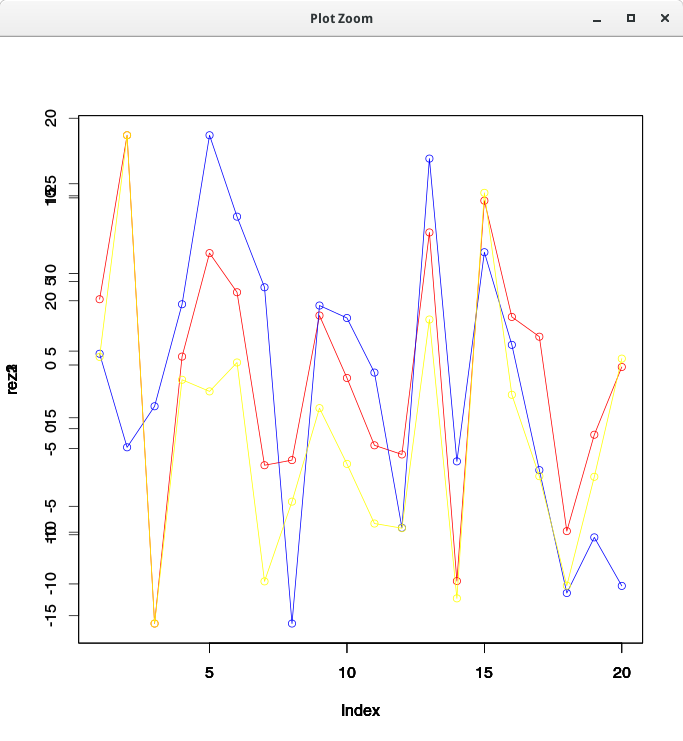
\includegraphics[width=\textwidth]{Images/mark10norm}
		\caption{Вывод графиков оценок для нормального распределения, выборка объёма 10.}
		\label{fig:mark10}
	
	\end{wrapfigure}
	
	\begin{wrapfigure}[13]{h}{\linewidth} 
		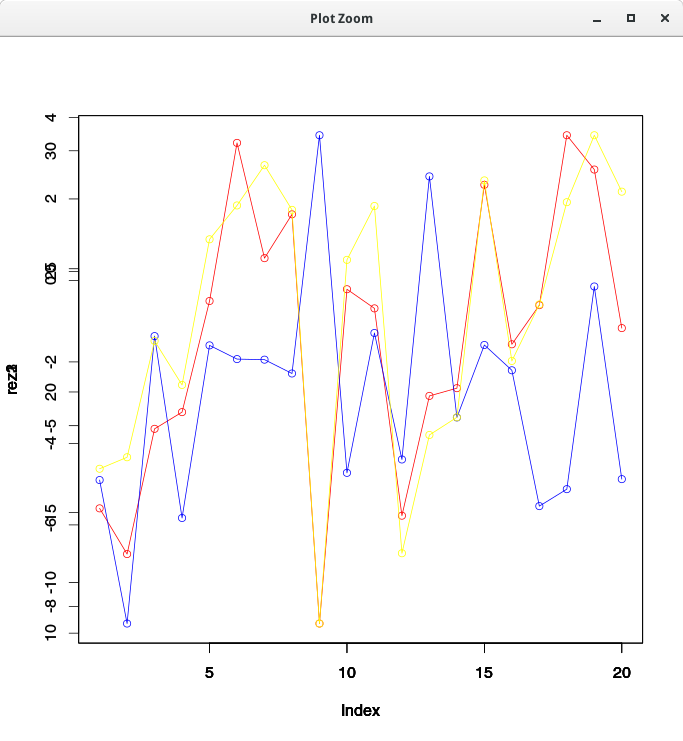
\includegraphics[width=\textwidth]{Images/mark40norm}
		\caption{Вывод графиков оценок для нормального распределения, выборка объёма 40.}
		\label{fig:mark10}
	
	\end{wrapfigure}
	
	\begin{wrapfigure}[13]{h}{\linewidth} 
		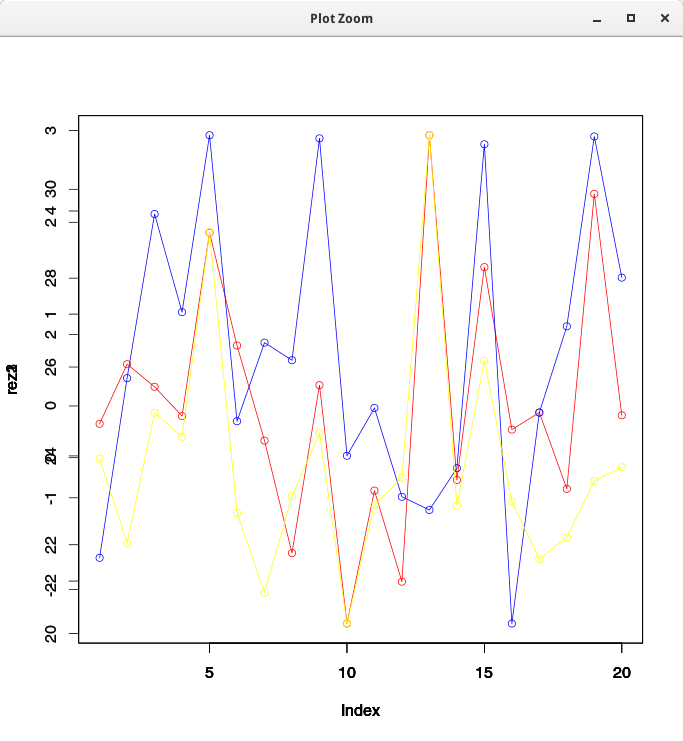
\includegraphics[width=\textwidth]{Images/mark160norm}
		\caption{Вывод графиков оценок для нормального экспоненциального, выборка объёма 160.}
		\label{fig:mark10}
	
	\end{wrapfigure}
%экспоненциальное	
	\begin{wrapfigure}[13]{h}{\linewidth} 
		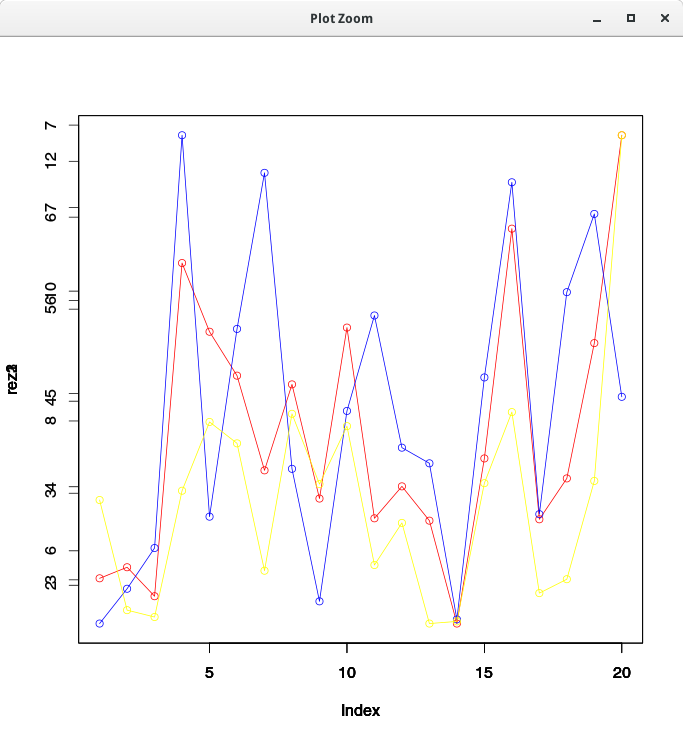
\includegraphics[width=\textwidth]{Images/mark10exp}
		\caption{Вывод графиков оценок для экспоненциального распределения, выборка объёма 10.}
		\label{fig:mark10}
	
	\end{wrapfigure}
	
	\begin{wrapfigure}[13]{h}{\linewidth} 
		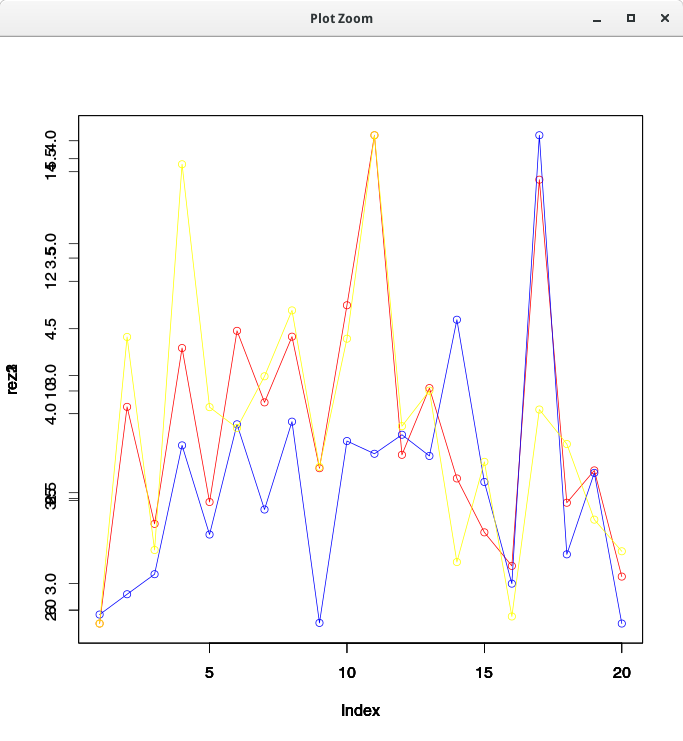
\includegraphics[width=\textwidth]{Images/mark40exp}
		\caption{Вывод графиков оценок для экспоненциального распределения, выборка объёма 40.}
		\label{fig:mark10}
	
	\end{wrapfigure}
	
	\begin{wrapfigure}[13]{h}{\linewidth} 
		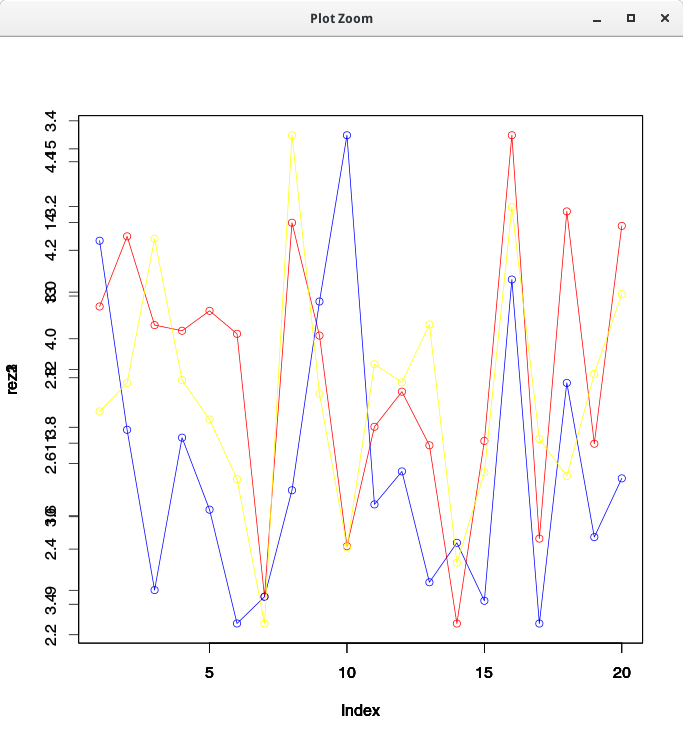
\includegraphics[width=\textwidth]{Images/mark160exp}
		\caption{Вывод графиков оценок для экспоненциального распределения, выборка объёма 160.}
		\label{fig:mark10}
	
	\end{wrapfigure}

\clearpage
	
\section{Графическое сравнение среднеквадратического отклонения трех оценок}
\subsection{Задание} 
Сравнить графически среднеквадратические отклонения трех оценок  для значений  n = 10, n = 40 и n = 160.
\subsection{Решение}
Для генерации выборки воспользуемся скриптами из предыдущей главы. Найдем среднеквадратичное отклонение и сохраним получившиеся значения:
\begin{itemize}
	\item Для n = 10:
	\lstset {language=R}
\begin{lstlisting}
p11 <- sd(rez1)
p12 <- sd(rez2)
p13 <- sd(rez3)
\end{lstlisting}
	\item Для n = 40:
	\lstset {language=R}
\begin{lstlisting}
p21 <- sd(rez1)
p22 <- sd(rez2)
p23 <- sd(rez3)
\end{lstlisting}
	\item Для n = 160:
	\lstset {language=R}
\begin{lstlisting}
p31 <- sd(rez1)
p32 <- sd(rez2)
p33 <- sd(rez3)
\end{lstlisting}
\end{itemize}
Сгенерируем график:
\lstset {language=R}
\begin{lstlisting}
mark10 <- c(p11, p12, p13)
mark40 <- c(p21, p22, p23)
mark160 <- c(p31, p32, p33)

plot(mark10, col = "red")
lines(mark10, col = "red")
par(new=T)
plot(mark40, col = "blue")
lines(mark40, col = "blue")
par(new=T)
plot(mark160, col = "yellow")
lines(mark160, col = "yellow")
par(new=F)
\end{lstlisting}

	\begin{wrapfigure}[13]{h}{0.5\linewidth} 
		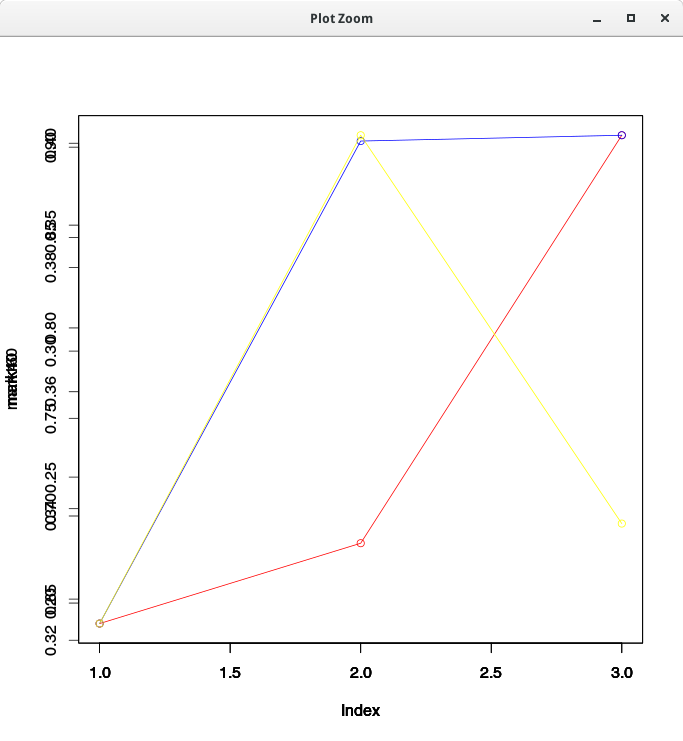
\includegraphics[width=0.5\textwidth]{Images/marksmark}
		\caption{Сравнение оценок.}
		\label{fig:mark10}
	
	\end{wrapfigure}
\end{document}
